\subsection{Testes}\label{sec:testes}
\subsubsection{Teste 1}
\begin{lstlisting}[frame=single,caption=Instância de teste 1,label=test1,escapeinside={\%*}{*)},inputencoding=utf8]
  3     // %*Número de estudantes*)
  5 1 2 // %*Ordem de inserção dos estudantes*)
  1     // %*Quantas consultas serão realizadas*)
  2     // %*Tutor do estudante 2*)
\end{lstlisting}

\begin{figure}[htb]
  \centering
  % dot -Gdpi=300 -Tpng test1.dot > test1.png
  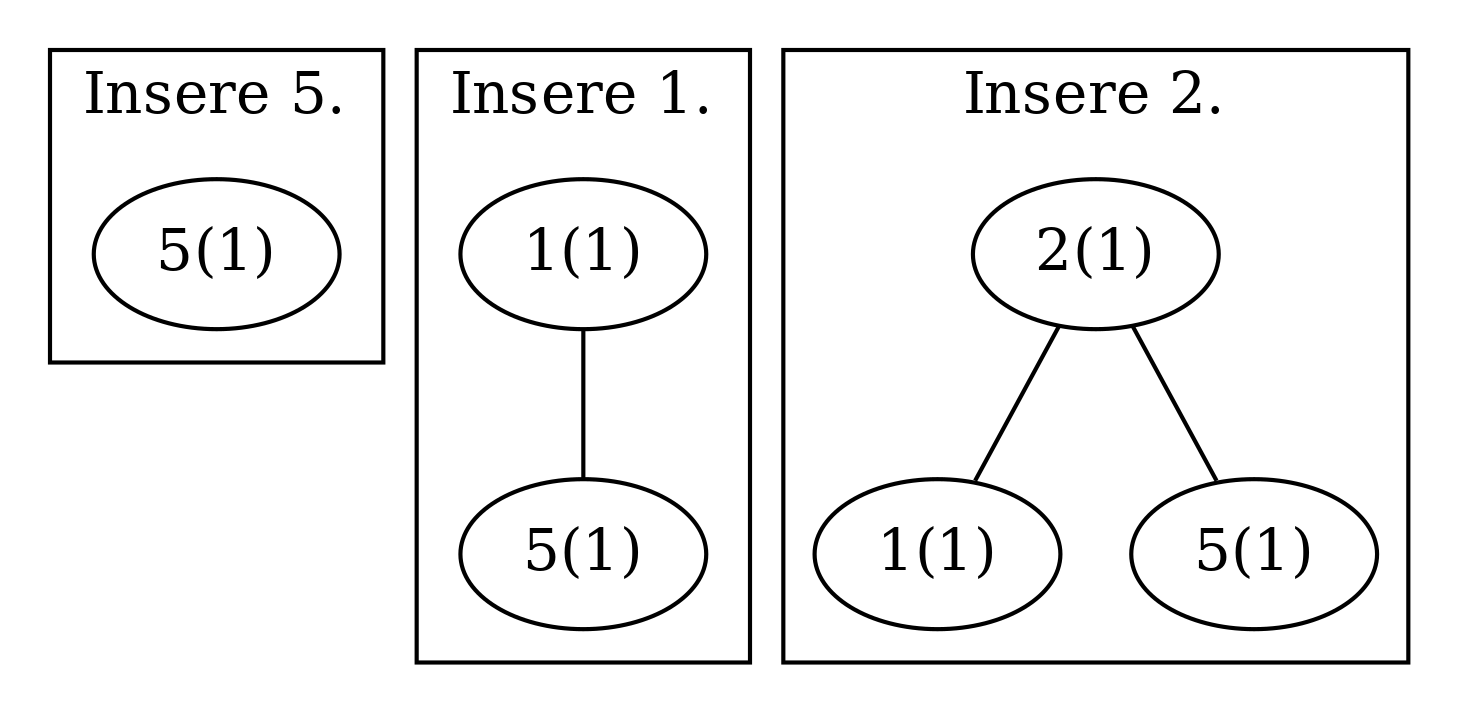
\includegraphics[width=0.5\linewidth]{test1.png}
  \caption{Inserção}
  \label{fig:test1}
\end{figure}

\subsubsection{Teste 2}
\begin{lstlisting}[frame=single,caption=Instância de teste 1,label=test1,escapeinside={\%*}{*)},inputencoding=utf8]
  5         // %*Número de estudantes*)
  3 1 4 2 5 // %*Ordem de inserção dos estudantes*)
  2         // %*Quantas consultas serão realizadas*)
  2 5       // %*Tutores dos estudantes 2 e 5*)
\end{lstlisting}

\begin{figure}[htb]
  \centering
  % dot -Gdpi=300 -Tpng test2.dot > test2.png
  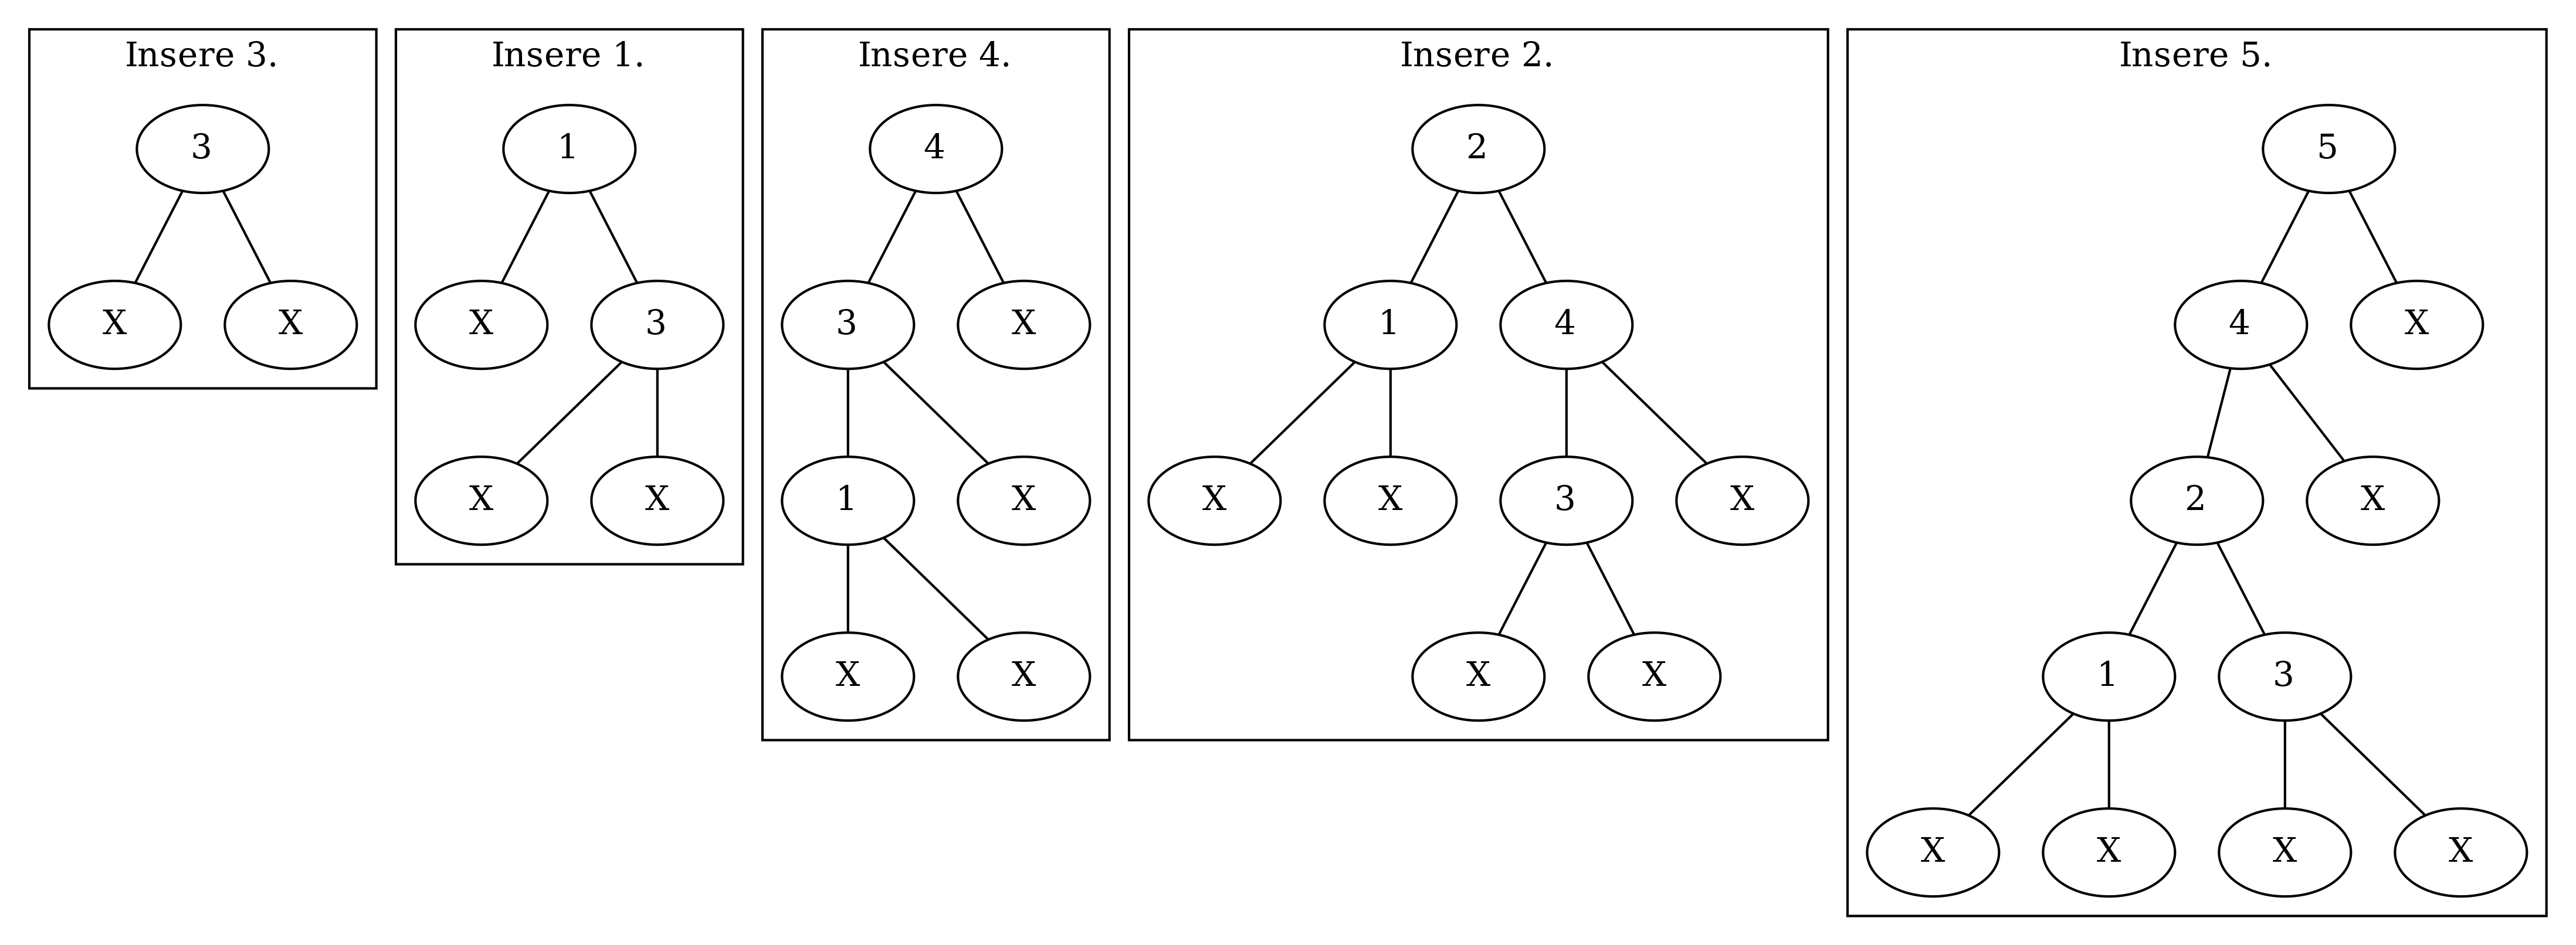
\includegraphics[width=\linewidth]{test2.png}
  \caption{Inserção}
  \label{fig:test1}
\end{figure}